\chapter{Рассмотрение существующих систем управления микроклиматом теплиц}

Среди существующих аналогов систем управления умными теплицами можно выделить следующие:

\begin{enumerate}
    \item AeroGarden
    \item Parrot Flower Power
    \item GreenIQ Smart Garden Hub
    \item Niwa
    \item Govee Smart Wi-Fi Термометр Гигрометр
    \item Mars Hydro Grow Tents
    \item Raspberry Pi Greenhouse Controller
    \item FarmBot
\end{enumerate}

\section{AeroGarden}

\begin{figure}[H]
    \centering
    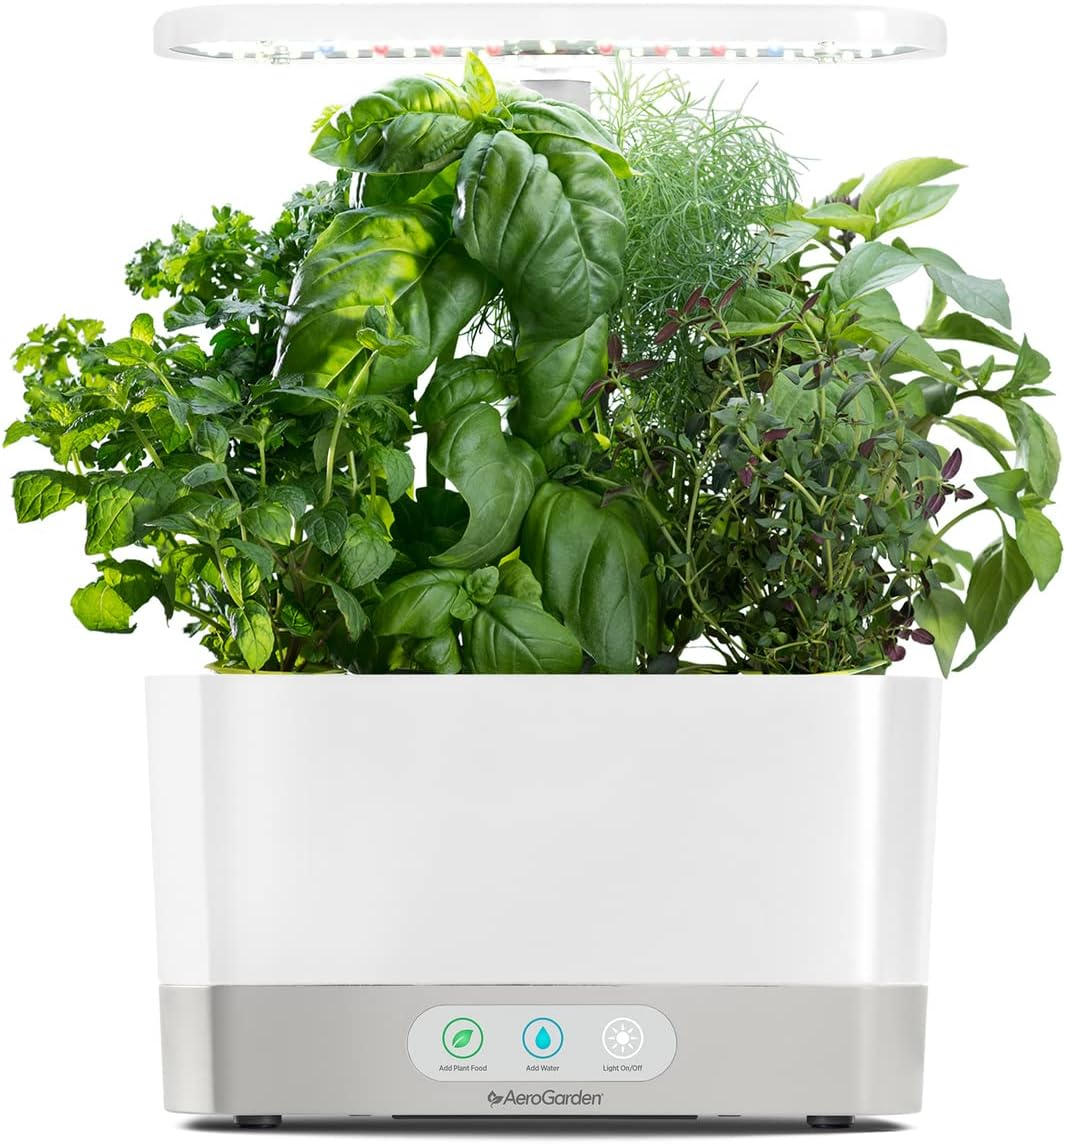
\includegraphics[scale=0.35]{images/AeroGarden.png}
    \caption{Система AeroGarden.}
    \label{fig:AeroGarden}
\end{figure}

AeroGarden --- это инновационная система гидропоники, разработанная для выращивания растений внутри дома. Эта теплица предоставляет возможность  выращивать свежие овощи, травы, цветы и другие растения в уникальных условиях~\cite{AeroGarden}.

Ключевые характеристики AeroGarden:

\begin{enumerate}
    \item гидропоника: AeroGarden использует гидропоническую систему, в которой растения растут без почвы. Вместо этого корни растений находятся в специальной среде, насыщенной водой и питательными веществами. Это способствует более эффективному поглощению питательных веществ и ускоряет рост растений;
    \item интегрированная LED-подсветка: одной из ключевых особенностей AeroGarden является интегрированная LED-подсветка, которая обеспечивает оптимальный спектр света для фотосинтеза и роста растений. Можно выбирать разные режимы освещения в зависимости от стадии роста растений;
    \item система автополива: AeroGarden автоматически поливает растения, поддерживая оптимальный уровень влажности для их роста;
    \item многофункциональные панели управления: AeroGarden обычно оснащается интуитивными панелями управления, которые позволяют настраивать параметры роста, включая освещение, полив и температуру;
    \item поддержка разнообразных растений: эта система подходит для выращивания широкого спектра растений. Выбор доступных семян и рассады может варьироваться в зависимости от модели AeroGarden;
    \item модели с различными размерами: AeroGarden предлагает разные модели с различными размерами и количеством мест для растений.
\end{enumerate}

Преимущества AeroGarden:

\begin{enumerate}
    \item круглогодичное выращивание;
    \item легкость в уходе.
\end{enumerate}

Недостатки AeroGarden:

\begin{enumerate}
    \item ограниченная вместимость;
    \item необходимость замены ламп.
\end{enumerate}

Заключение:

AeroGarden представляет собой инновационную систему гидропоники, которая позволяет выращивать свежие растения внутри помещения круглый год. С его интегрированной LED-подсветкой, автополивом и многофункциональными панелями управления, AeroGarden обеспечивает идеальные условия для роста растений.

\section{Parrot Flower Power}

\begin{figure}[H]
    \centering
    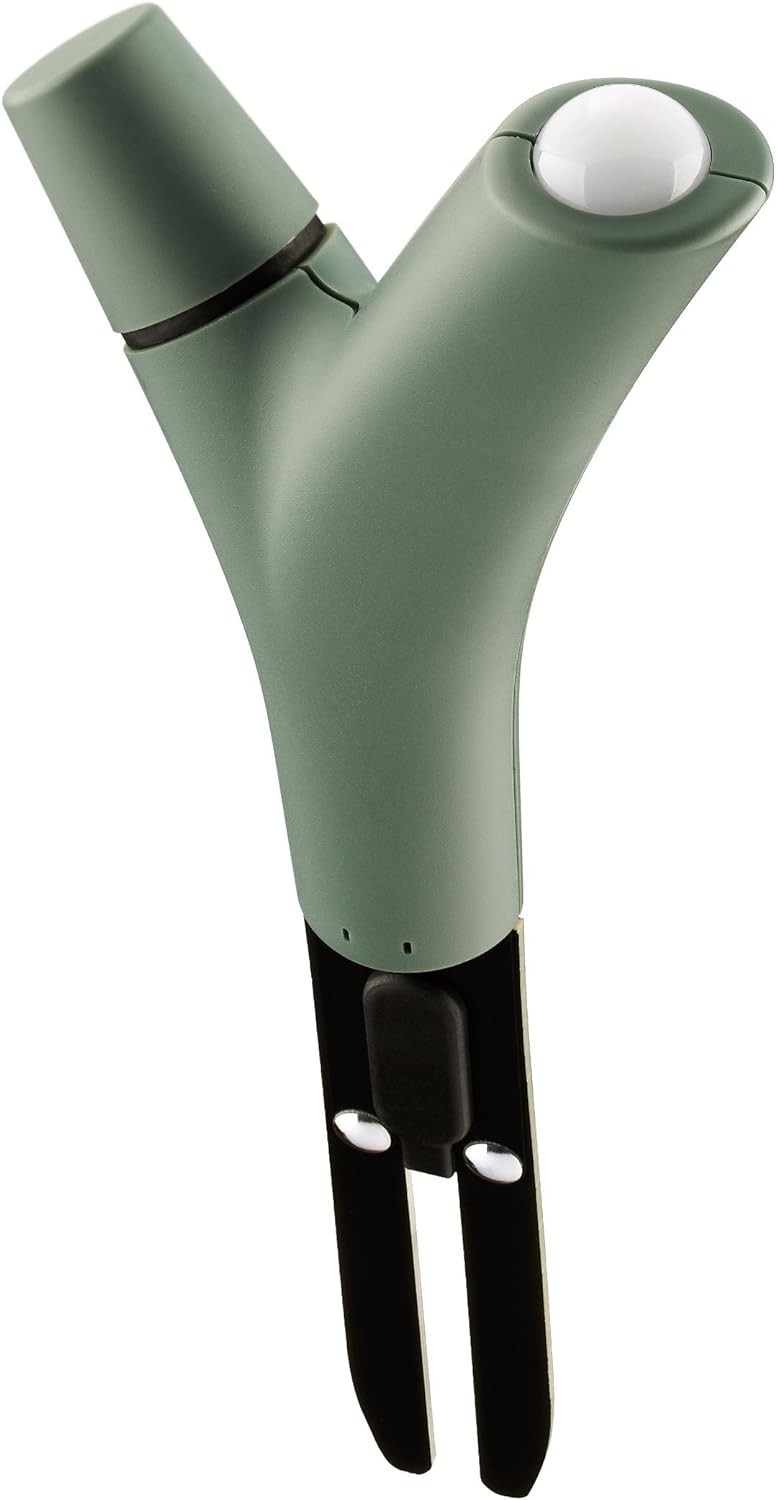
\includegraphics[scale=0.35]{images/ParrotFlowerPower.png}
    \caption{Система Parrot Flower Power.}
    \label{fig:ParrotFlowerPower}
\end{figure}

Parrot Flower Power --- это умное устройство, созданное для того, чтобы улучшить заботу за растениями, независимо от того, растут ли они внутри помещения или на открытом воздухе. Это компактное устройство позволяет более эффективно следить за здоровьем растений, обеспечивая оптимальные условия для роста~\cite{ParrotFlowerPower}. 

Основные характеристики:

\begin{enumerate}
    \item измерение важных параметров: Parrot Flower Power оснащен датчиками, которые измеряют несколько важных параметров, включая влажность почвы, уровень света, температуру и уровень удобрений;
    \item синхронизация с мобильным приложением: устройство отправляет собранные данные на смартфон через беспроводное соединение, таким образом можно отслеживать состояние растений в реальном времени;
    \item рекомендации и уведомления: мобильное приложение предоставляет рекомендации и уведомления на основе данных, помогая принимать правильные решения о том, как ухаживать за растениями.
\end{enumerate}

Преимущества:

\begin{enumerate}
    \item оптимизация ухода;
    \item совместимость с разными растениями;
    \item поддержка мобильного приложения.
\end{enumerate}

Недостатки:

\begin{enumerate}
    \item требуется аккумулятор;
    \item ограниченная связь: устройству требует Bluetooth-соединения со смартфоном.
\end{enumerate}

Заключение:

Parrot Flower Power --- это отличное устройство, которое предоставляет не только информацию о состоянии растений, но и практические советы для улучшения условий и роста. 

\section{GreenIQ Smart Garden Hub}

\begin{figure}[H]
    \centering
    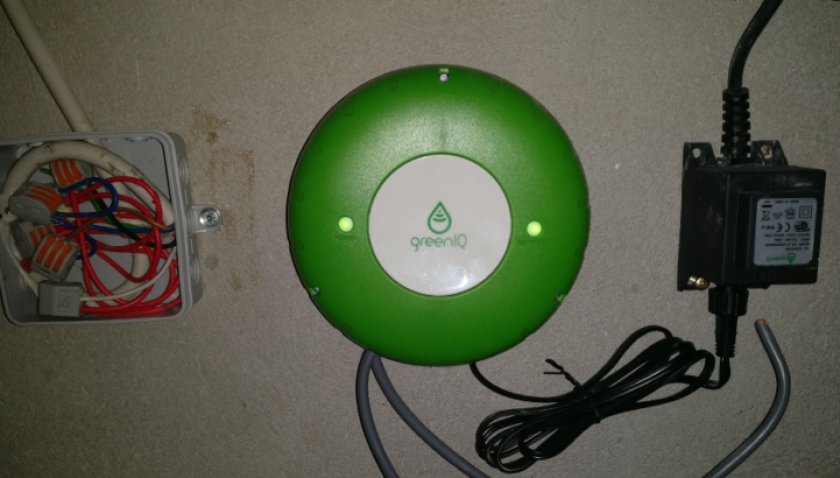
\includegraphics[scale=0.5]{images/GreenIQSmartGardenHub.png}
    \caption{Система GreenIQ Smart Garden Hub.}
    \label{fig:GreenIQSmartGardenHub}
\end{figure}

GreenIQ Smart Garden Hub --- это умное устройство, разработанное для автоматизации полива сада или ландшафта. Он предоставляет множество функций для оптимизации полива растений~\cite{GreenIQ}.

Ключевые характеристики:

\begin{enumerate}
    \item подключение к Wi-Fi: GreenIQ подключается к Wi-Fi-сети, что позволяет удаленно управлять им через мобильное приложение;
    \item метеоданные и адаптивный полив: устройство использует метеоданные в реальном времени, такие как прогноз погоды, температура и осадки, чтобы определить оптимальное расписание полива;
    \item совместимость с различными системами полива: GreenIQ совместим с различными системами полива, включая системы капельного полива, спринклеры и шланги. Есть возможность интегрировать его в вашу существующую систему или создать новую;
    \item поддержка множества зон: это устройство способно управлять поливом в нескольких зонах сада независимо друг от друга. Можно настроить разное расписание и длительность полива для каждой зоны в зависимости от потребностей растений;
    \item интеграция с дополнительными датчиками: можно добавить дополнительные датчики, такие как датчики влажности почвы или солнечной радиации, чтобы получить более точную информацию о состоянии сада и управлять поливом на основе этих данных;
    \item мобильное приложение: GreenIQ предоставляет удобное мобильное приложение (доступное для устройств на iOS и Android), с помощью которого можно настроить параметры полива, мониторить статистику и получать уведомления.
\end{enumerate}

Преимущества:

\begin{enumerate}
    \item экономия воды;
    \item удобство управления;
    \item интеграция с другими системами.
\end{enumerate}

Недостатки:

\begin{enumerate}
    \item зависимость от Wi-Fi.
\end{enumerate}

Заключение:

GreenIQ Smart Garden Hub --- это отличное умное устройство для того, чтобы автоматизировать полив сада и обеспечить оптимальные условия для роста растений. 

\section{Niwa}

\begin{figure}
    \centering
    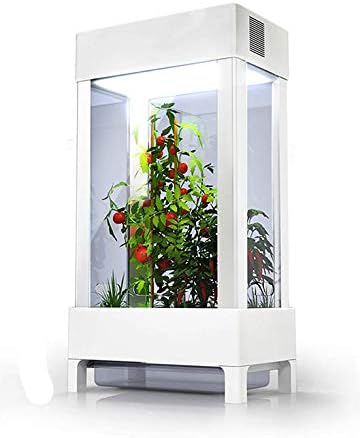
\includegraphics{images/Niwa.png}
    \caption{Система Niwa.}
    \label{fig:Niwa}
\end{figure}

Niwa --- это умная теплица, разработанная для выращивания растений внутри помещения с использованием передовых технологий и автоматизированных систем. Эта система позволяет создать идеальные условия для роста различных растений, включая овощи, травы и цветы, вне зависимости от времени года и климата~\cite{Niwa}. 

Ключевые характеристики Niwa:

\begin{enumerate}
    \item управление через мобильное приложение: основной элемент управления Niwa --- мобильное приложение, которое позволяет контролировать и настраивать параметры окружающей среды в теплице. Это включает в себя уровень освещенности, температуру, влажность, и даже подачу воды;
    \item сенсоры и контроль: Niwa оснащена множеством сенсоров для непрерывного мониторинга условий в теплице. Это включает в себя датчики температуры, влажности, уровня $CO_2$ и даже качества воды. Собранные данные используются для автоматической коррекции параметров;
    \item LED-подсветка: Niwa предлагает встроенную LED-подсветку, которая регулируется с помощью мобильного приложения. Можно настроить спектр и интенсивность света в соответствии с потребностями конкретных растений;
    \item автополив: встроенная система автополива позволяет поддерживать оптимальный уровень влажности в почве;
    \item интеграция с Wi-Fi: Niwa поддерживает Wi-Fi-связь, что позволяет управлять теплицей из любой точки мира через интернет;
    \item система ростовых кассет: Niwa поставляется с модульной системой ростовых кассет, которые позволяют легко выращивать разнообразные растения.
\end{enumerate}

Преимущества Niwa:

\begin{enumerate}
    \item оптимальные условия для роста;
    \item удобное управление;
    \item интеграция с Wi-Fi;
    \item модульность.
\end{enumerate}

Недостатки Niwa:

\begin{enumerate}
    \item необходимость в стабильном Wi-Fi;
    \item ограниченное пространство.
\end{enumerate}

Заключение:

Niwa --- это выдающаяся умная теплица, которая предоставляет возможность выращивать растения внутри помещения с минимумом усилий и максимумом контроля. Её возможности по мониторингу и настройке окружающей среды делают её идеальным выбором.

\section{Govee Smart Wi-Fi Термометр Гигрометр}

\begin{figure}[H]
    \centering
    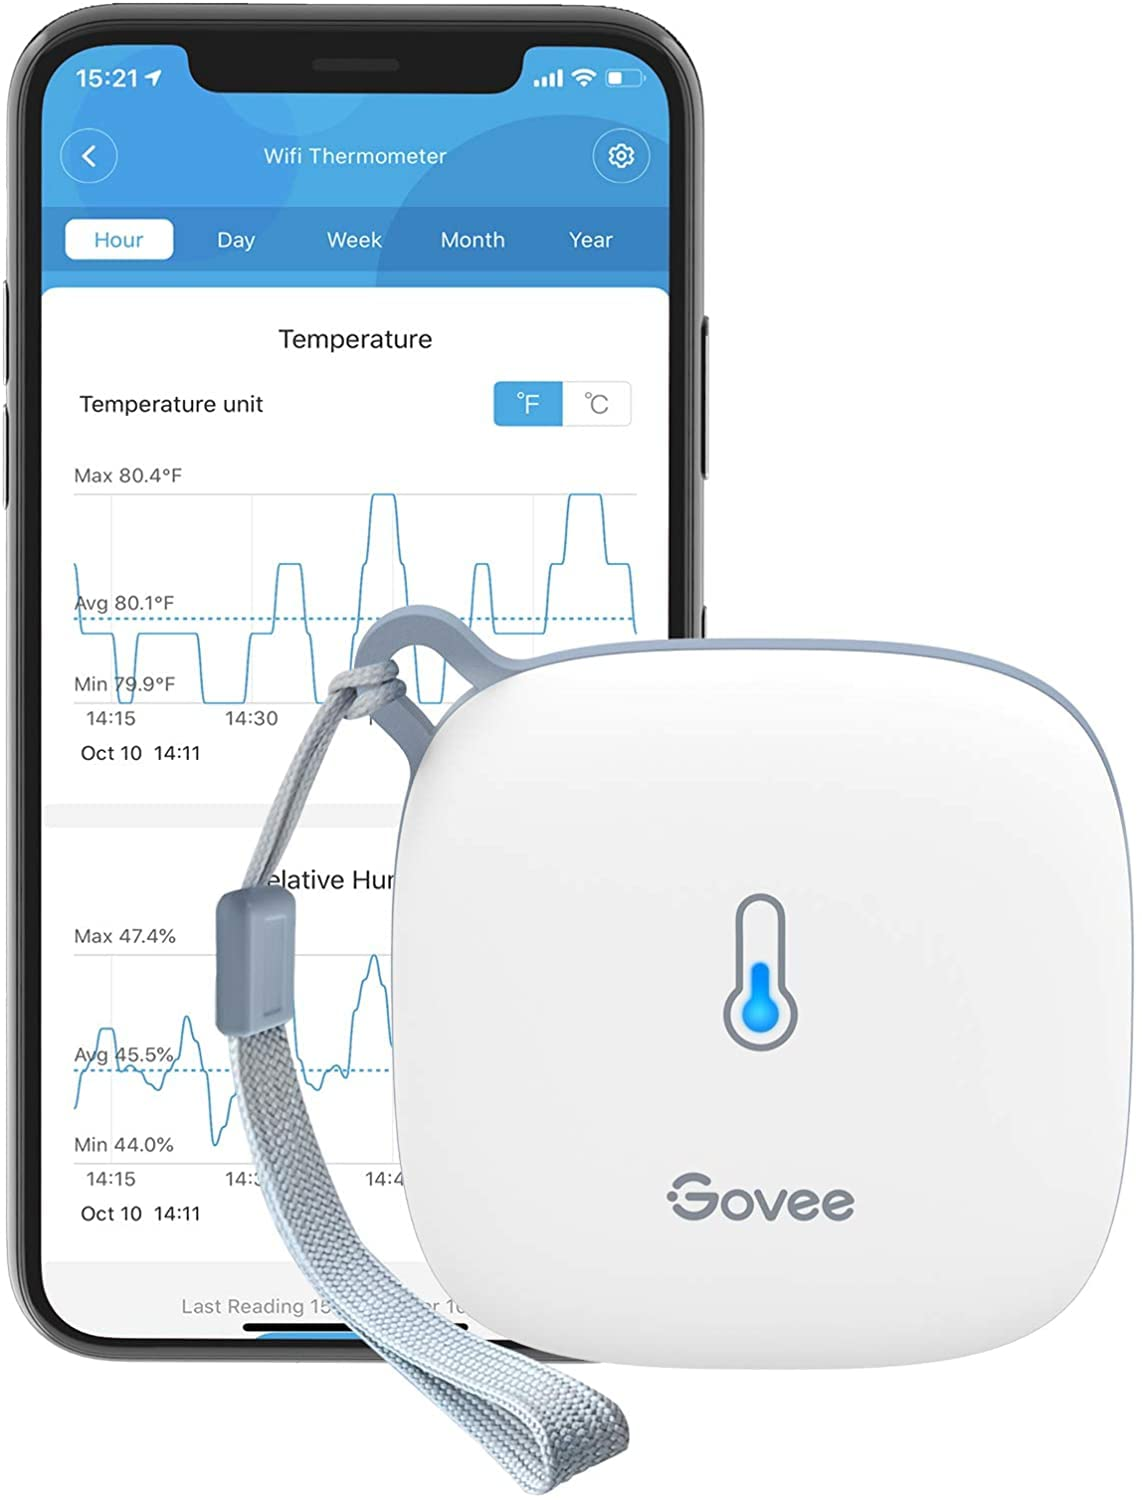
\includegraphics[scale=0.25]{images/GoveeSmartWiFi.png}
    \caption{Система Govee Smart Wi-Fi Термометр Гигрометр.}
    \label{fig:GoveeSmartWiFi}
\end{figure}

Govee Smart Wi-Fi Термометр Гигрометр (Govee Smart Wi-Fi Thermometer Hygrometer) --- это умное устройство, предназначенное для мониторинга температуры и влажности в помещении~\cite{Govee}.

Ключевые характеристики:

\begin{enumerate}
    \item измерение температуры и влажности: Govee Smart Wi-Fi Термометр Гигрометр точно измеряет температуру и влажность внутри помещения;
    \item Wi-Fi-подключение: устройство подключается к вашей домашней сети Wi-Fi, что позволяет вам мониторить данные удаленно через мобильное приложение;
    \item мобильное приложение: Govee предоставляет бесплатное мобильное приложение, которое позволяет в режиме реального времени отслеживать данные о температуре и влажности, а также получать уведомления, когда они выходят за пределы заданных диапазонов;
    \item графики и история данных: приложение также предоставляет графики и историю данных, что позволяет анализировать изменения температуры и влажности в течение времени;
    \item настройка предупреждений: можно настроить предупреждения, чтобы получать уведомления, когда температура или влажность выходят за заданные пределы.;
    \item совместимость с голосовыми помощниками: Govee Smart Wi-Fi Термометр Гигрометр совместим с голосовыми помощниками, такими как Amazon Alexa и Google Assistant, что позволяет получать информацию о температуре и влажности, используя голосовые команды.
\end{enumerate}

Преимущества:

\begin{enumerate}
    \item дистанционный мониторинг;
    \item предупреждения и уведомления;
    \item голосовая интеграция.
\end{enumerate}

Недостатки:

\begin{enumerate}
    \item требуется Wi-Fi-соединение;
    \item зависимость от питания.
\end{enumerate}

Заключение:

Govee Smart Wi-Fi Термометр Гигрометр --- это удобное и надежное устройство для мониторинга температуры и влажности в помещении. Он предоставляет множество полезных функций, такие как дистанционное управление, уведомления и голосовая интеграция.

\section{Mars Hydro Grow Tents}

\begin{figure}
    \centering
    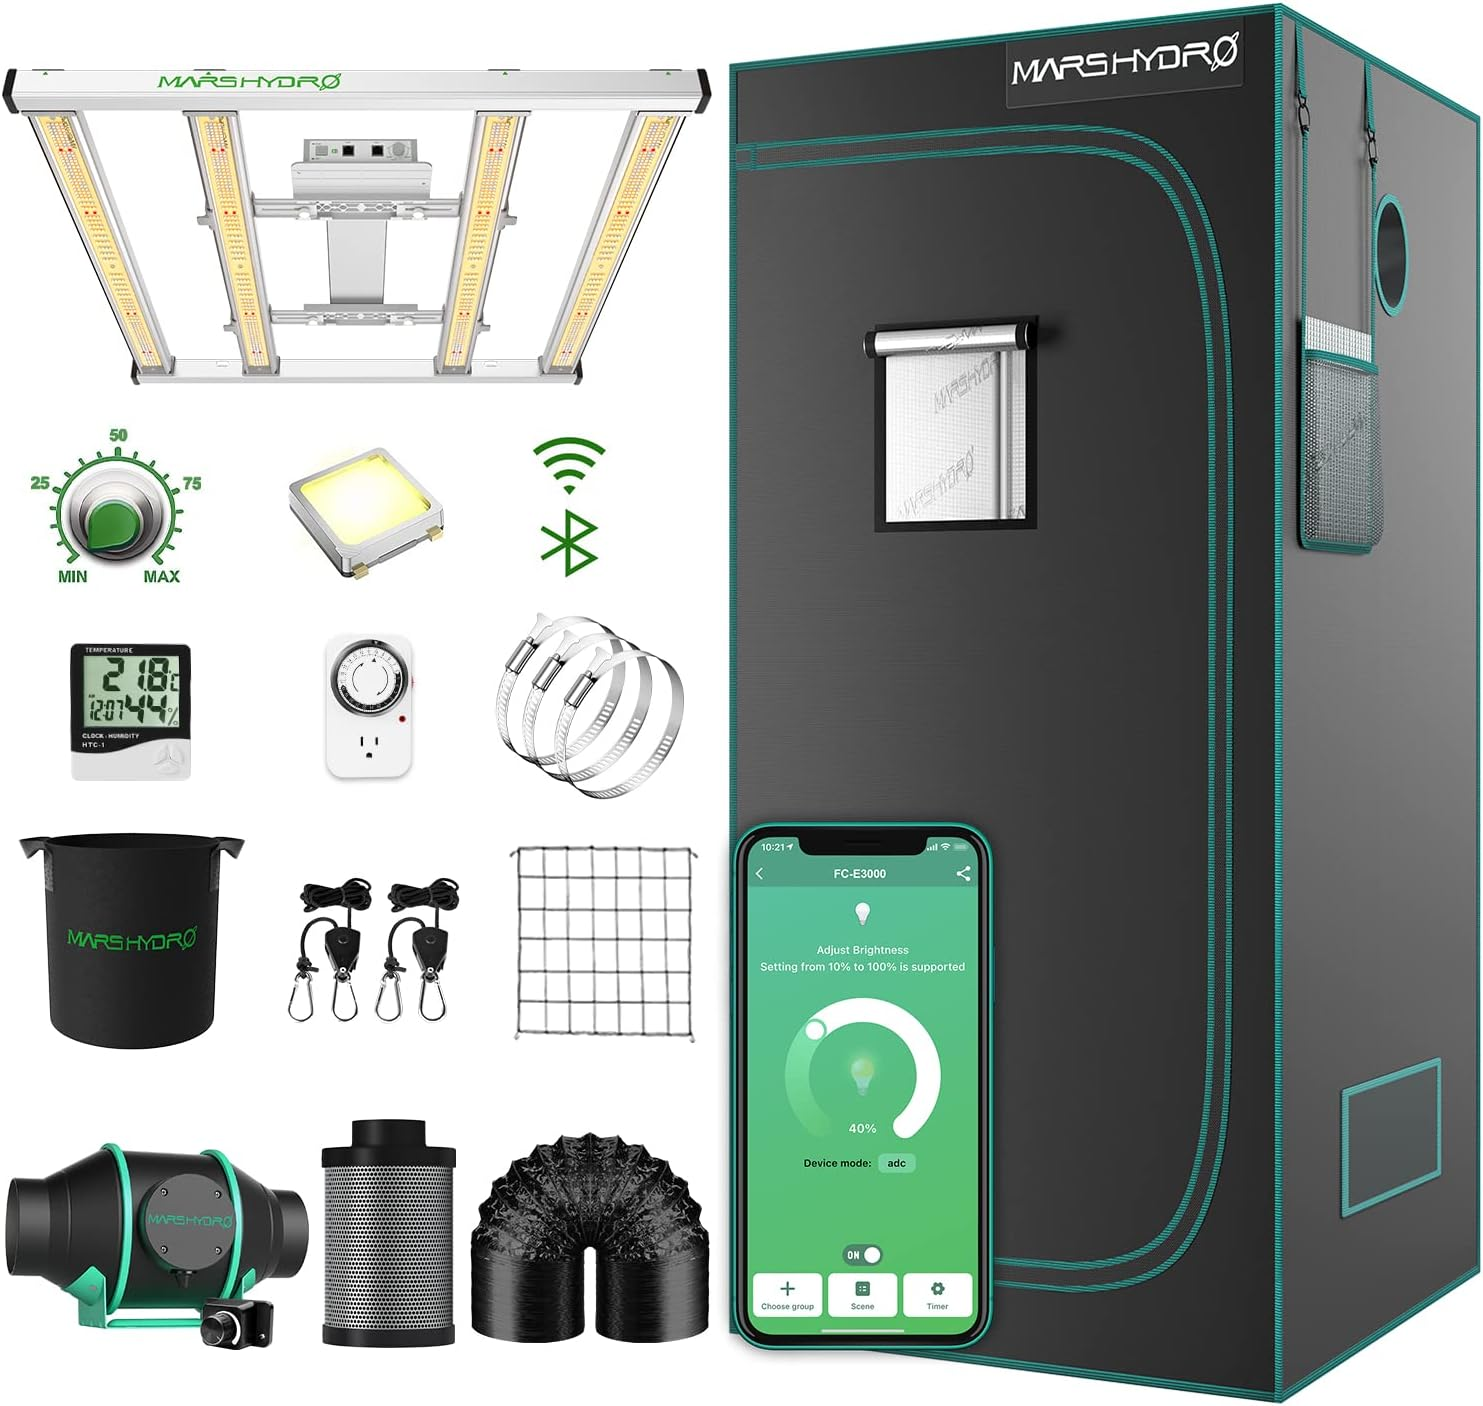
\includegraphics[scale=0.3]{images/MarsHydroGrowTents.png}
    \caption{Система Mars Hydro Grow Tents.}
    \label{fig:MarsHydroGrowTents}
\end{figure}

Mars Hydro Grow Tents --- это семейство умных теплиц, разработанных компанией Mars Hydro, которые предоставляют возможность выращивать растения внутри помещения с оптимальными условиями~\cite{Mars}.

Основные характеристики Mars Hydro Grow Tents:

\begin{enumerate}
    \item LED-подсветка: все теплицы Mars Hydro оснащены мощными LED-панелями, специально разработанными для растений. Эти панели обеспечивают растениям необходимый спектр света для фотосинтеза;
    \item системы вентиляции: каждая теплица оборудована системой вентиляции, которая обеспечивает постоянное поступление свежего воздуха и выводит тепловые избытки и запахи;
    \item конструкция и материалы: теплицы Mars Hydro выполнены из высококачественных материалов, обладающих хорошей теплоизоляцией и устойчивостью к влаге. Их прочная конструкция предотвращает проникновение света извне;
    \item простор и доступ: теплицы предлагают разные размеры, позволяя выбрать подходящий вариант в зависимости от потребностей. Они также оборудованы множеством дверей, окон и отверстий для кабелей, что облегчает доступ к растениям и обслуживание.
\end{enumerate}

Преимущества:

\begin{enumerate}
    \item контролируемые условия роста;
    \item множество доступных размеров.
\end{enumerate}

Недостатки:

\begin{enumerate}
    \item расход электроэнергии: хотя LED-подсветка эффективнее, она все равно потребляет электроэнергию, что может повысить электрозатраты;
    \item ограничения по размеру помещения: для ограниченного пространства, большие теплицы Mars Hydro могут не подходить.
\end{enumerate}

Заключение:

В целом, Mars Hydro Grow Tents предоставляют многочисленные преимущества для того, чтобы выращивать растения внутри помещения. Позволяют создать идеальные условия для роста, обеспечивают высокий урожай и контролируемость процесса. 

\section{Raspberry Pi Greenhouse Controller}

\begin{figure}[H]
    \centering
    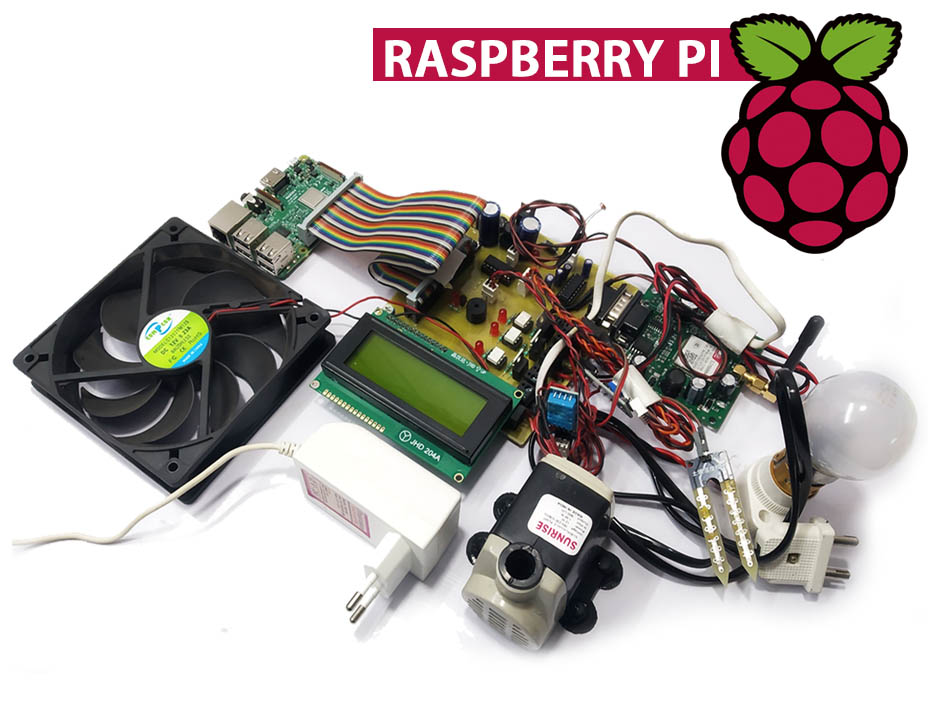
\includegraphics[scale=0.4]{images/RaspberryPiGreenhouseController.png}
    \caption{Система Raspberry Pi Greenhouse Controller.}
    \label{fig:RaspberryPiGreenhouseController}
\end{figure}

Raspberry Pi Greenhouse Controller --- это проект, предоставляющий возможность создать умную теплицу с использованием одноплатного компьютера Raspberry Pi. Этот устройство позволяет автоматизировать и контролировать различные аспекты выращивания растений, включая температуру, влажность, освещение и полив~\cite{Raspberry}. 

Основные характеристики:

\begin{enumerate}
    \item Raspberry Pi совместимость: Raspberry Pi --- это мини-компьютер с открытым исходным кодом, который можно легко настроить и программировать. Он предоставляет широкие возможности для создания пользовательских умных систем, включая умные теплицы;
    \item датчики и сенсоры: Raspberry Pi Greenhouse Controller обычно включает в себя разнообразные датчики и сенсоры, такие как датчики температуры, влажности почвы, влажности воздуха, освещенности и другие;
    \item актуаторы: устройство может быть интегрировано с различными актуаторами, такими как насосы для полива, вентиляторы для вентиляции, и даже системы управления освещением;
    \item интеграция с Интернетом: Raspberry Pi Greenhouse Controller может быть подключен к интернету, что позволяет удаленно управлять и мониторить теплицу через веб-интерфейс или мобильное приложение;
    \item программируемость: одним из главных преимуществ этой системы является ее программируемость. Можно использовать различные языки программирования, такие как Python, для написания скриптов и автоматизировать процессы управления теплицей.
\end{enumerate}

Преимущества:

\begin{enumerate}
    \item гибкость: возможность иметь полный контроль над конфигурацией и функциональностью умной теплицы;
    \item обновления и улучшения: Raspberry Pi Greenhouse Controller может быть легко обновлен и модифицирован по мере необходимости, что позволяет внедрять новые функции и улучшения.
\end{enumerate}

Недостатки:

\begin{enumerate}
    \item технические знания: создание и настройка умной теплицы на основе Raspberry Pi может потребовать определенных технических навыков в программировании и электронике;
    \item зависимость от электропитания: Raspberry Pi Greenhouse Controller требует постоянного электропитания, поэтому при отключении электроэнергии могут возникнуть проблемы с управлением.
\end{enumerate}

Заключение:

В целом, Raspberry Pi Greenhouse Controller --- это отличная опция для того, чтобы создать умную теплицу при наличии технических навыков для этого. 

\section{FarmBot}

\begin{figure}[H]
    \centering
    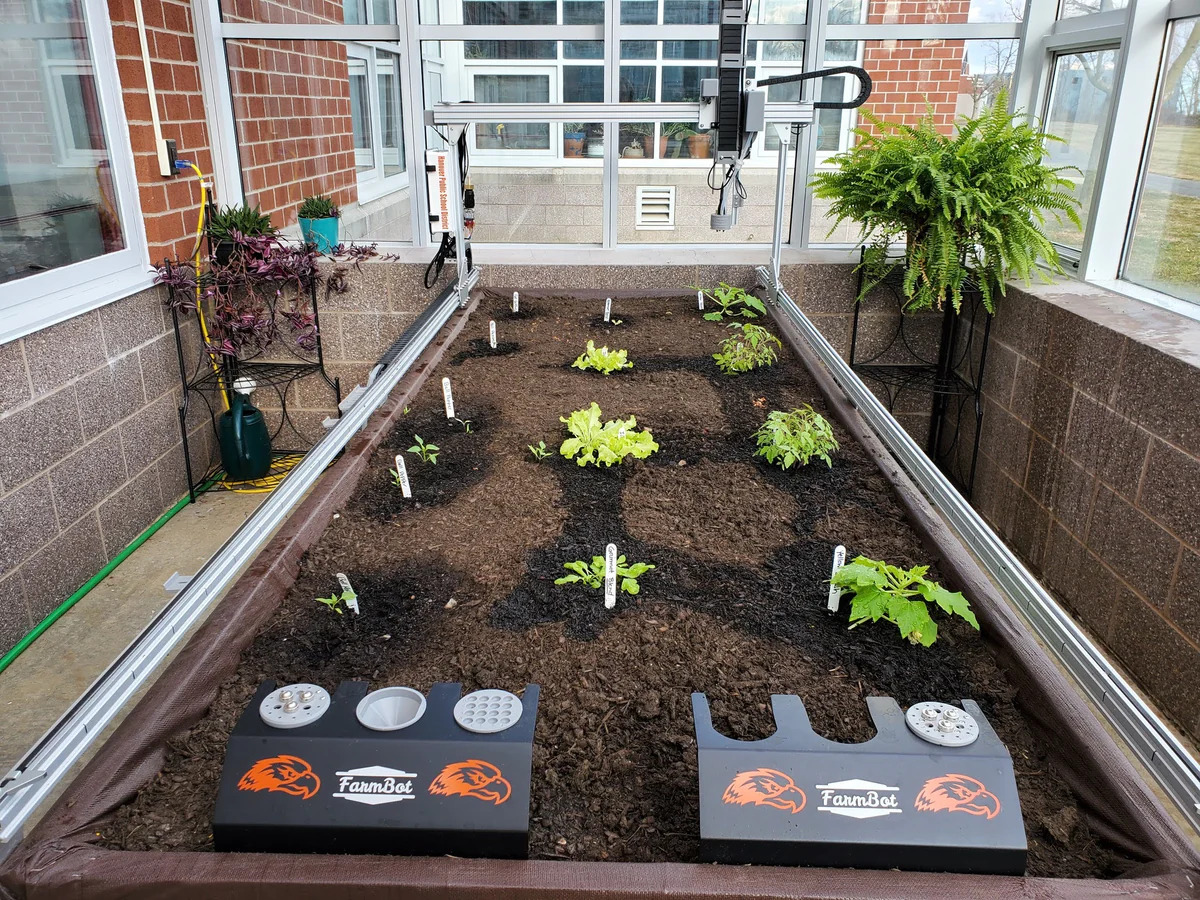
\includegraphics[scale=0.3]{images/FarmBot.png}
    \caption{Система FarmBot.}
    \label{fig:FarmBot}
\end{figure}

FarmBot --- это инновационная и мощная система для автоматизации процессов садоводства и сельского хозяйства. Она предназначена для создания и управления автоматизированными садами и огородами, обеспечивая точное и эффективное выращивание растений~\cite{FarmBot}.

Основные характеристики:

\begin{enumerate}
    \item роботизированная система: FarmBot состоит из робота, который перемещается по садовому участку и выполняет различные задачи, такие как сеять семена, поливать, удобрять и ухаживать за растениями. Робот оснащен специальным инструментом для точной работы с почвой;
    \item вертикальная и горизонтальная мобильность: FarmBot может двигаться как в вертикальном, так и в горизонтальном направлении, что позволяет ему работать на больших сельскохозяйственных участках и в теплицах;
    \item подключение к интернету: FarmBot подключается к Интернету, что позволяет управлять им удаленно через веб-интерфейс;
    \item оптическая система распознавания растений: FarmBot оснащен камерой и оптической системой, которая может распознавать растения и определять их состояние;
    \item поддержка множества растений: FarmBot подходит для выращивания разнообразных культур, включая овощи, цветы, злаки и другие.
\end{enumerate}

Преимущества:

\begin{enumerate}
    \item автоматизация и точность;
    \item экономия воды и удобрений;
    \item масштабируемость: можно настраивать FarmBot под размер вашего участка и потребности в выращивании;
    \item мониторинг и управление через Интернет.
\end{enumerate}

Недостатки:

\begin{enumerate}
    \item сложность установки и настройки: установка и настройка FarmBot могут потребовать определенных технических навыков;
    \item зависимость от интернет-соединения.
\end{enumerate}

Заключение:

FarmBot представляет собой революционную систему для автоматизации садоводства и сельского хозяйства. Он объединяет в себе роботизированные технологии, оптическое распознавание и возможность удаленного управления, что делает его мощным инструментом для оптимизации процессов выращивания растений. 